% Ujjwal Rail -- AI-Powered Train Travel Assistant
% HCLTech AI Engineer Hackathon -- technical presentation
% Compiled with: tectonic presentation.tex
\documentclass[aspectratio=169]{beamer}

\usepackage{lmodern}
\usepackage[T1]{fontenc}
\usepackage[utf8]{inputenc}
\usepackage{graphicx}
\usepackage{tikz}
\usetikzlibrary{arrows.meta,positioning,fit,backgrounds,shadows}
\usepackage{booktabs}
\usepackage{array}
\usepackage{textpos}
\usepackage{relsize}

% ---------------------------------------------------------------------
% Colour palette: dark navy background, blue/cyan accents, white text
% ---------------------------------------------------------------------
\definecolor{bgNavy}{RGB}{9,14,28}
\definecolor{panelNavy}{RGB}{15,22,42}
\definecolor{panelNavy2}{RGB}{20,30,54}
\definecolor{lineNavy}{RGB}{40,54,86}
\definecolor{accentCyan}{RGB}{56,201,255}
\definecolor{accentBlue}{RGB}{66,133,244}
\definecolor{accentBlueDark}{RGB}{37,86,180}
\definecolor{textWhite}{RGB}{244,247,252}
\definecolor{textGray}{RGB}{158,172,198}
\definecolor{warnAmber}{RGB}{245,180,80}
\definecolor{okGreen}{RGB}{90,210,160}

\setbeamertemplate{navigation symbols}{}
\setbeamercolor{background canvas}{bg=bgNavy}
\setbeamercolor{normal text}{fg=textWhite,bg=bgNavy}
\setbeamercolor{frametitle}{fg=textWhite,bg=bgNavy}
\setbeamercolor{title}{fg=textWhite}
\setbeamercolor{itemize item}{fg=accentCyan}
\setbeamercolor{itemize subitem}{fg=accentBlue}
\setbeamertemplate{itemize item}{\color{accentCyan}\scriptsize$\blacktriangleright$}
\setbeamertemplate{itemize subitem}{\color{accentBlue}\tiny$\bullet$}
\setbeamerfont{frametitle}{size=\Large,series=\bfseries}
\setbeamerfont{framesubtitle}{size=\normalsize,series=\mdseries}
\setbeamertemplate{frametitle}{}
\setbeamersize{text margin left=9mm,text margin right=9mm}

\newcommand{\sectiontag}[1]{\textcolor{accentCyan}{\scriptsize\textsf{#1}}}

% Custom frame title bar, drawn once per frame via a TikZ background
\newcommand{\framebar}[2]{%
  \begin{tikzpicture}[remember picture,overlay]
    \shade[left color=accentBlueDark,right color=accentCyan] (current page.north west)
      ++(0,-0.02\paperheight) rectangle ++(\paperwidth,0.012\paperheight);
  \end{tikzpicture}%
  \vspace{-2mm}
  {\sectiontag{#2}}\\[1mm]
  {\usebeamerfont{frametitle}\usebeamercolor[fg]{frametitle}#1}
  \vspace{2mm}\hrule height 0.4pt \color{lineNavy}
  \vspace{3mm}
}

% A small rounded "card" box. Content is wrapped in a real minipage
% (not just a TikZ node "text width") so itemize/tabular inside it
% build their boxes the normal, reliable LaTeX way.
\newcommand{\cardbox}[3][panelNavy]{%
  \begin{tikzpicture}
    \node[draw=lineNavy,rounded corners=3pt,fill=#1,inner sep=8pt,
          drop shadow={shadow xshift=0pt,shadow yshift=-1pt,opacity=0.35}]
      {\begin{minipage}{#2}\color{textWhite}\footnotesize #3\end{minipage}};
  \end{tikzpicture}%
}

% Status pill: implemented / partial / mocked / future
\newcommand{\pill}[2][okGreen]{\tikz[baseline=-0.6ex]{\node[draw=#1,fill=#1!18,rounded corners=6pt,inner sep=2.2pt,font=\tiny\bfseries,text=#1]{#2};}}
\newcommand{\pillDone}{\pill[okGreen]{IMPLEMENTED}}
\newcommand{\pillPartial}{\pill[accentCyan]{PARTIAL}}
\newcommand{\pillMock}{\pill[warnAmber]{MOCKED (TEST FAKE)}}
\newcommand{\pillFuture}{\pill[textGray]{FUTURE WORK}}

\title{Ujjwal Rail}
\subtitle{AI-Powered Train Travel Assistant}
\date{21 November 2026}

\begin{document}

% ======================================================================
\begin{frame}[plain]
  \begin{tikzpicture}[remember picture,overlay]
    \shade[top color=panelNavy2,bottom color=bgNavy] (current page.north west) rectangle (current page.south east);
    \shade[left color=accentBlueDark,right color=accentCyan] (current page.north west) ++(0,-0.015\paperheight) rectangle ++(\paperwidth,0.02\paperheight);
  \end{tikzpicture}
  \vspace{18mm}
  \begin{center}
    {\fontsize{40}{44}\selectfont\color{textWhite}\textbf{Ujjwal Rail}}\\[3mm]
    {\Large\color{accentCyan}AI-Powered Train Travel Assistant}\\[8mm]
    {\small\color{textGray}HCLTech \textbf{Future Ready AI Engineer} Hackathon}\\[2mm]
    {\small\color{textGray}Grounded answers $\cdot$ deterministic calculations $\cdot$ safe confirmed actions}\\[10mm]
    
\begin{tikzpicture}
      \node[draw=lineNavy,rounded corners=4pt,fill=panelNavy,inner sep=10pt] {%
        \color{textWhite}\footnotesize
        \begin{tabular}{@{}l l@{}}
          \textcolor{accentCyan}{\textbf{Team workstreams:}} & RAG $\cdot$ Backend \& APIs $\cdot$ AI/LLM \& Orchestration $\cdot$ Frontend \& UX $\cdot$ Data, Testing \& Evaluation \\
        \end{tabular}
      };
    \end{tikzpicture}\\[6mm]
    {\footnotesize\color{textGray}21 November 2026}
  \end{center}
\end{frame}

% ======================================================================
\begin{frame}{}
  \framebar{Problem Statement}{01 -- WHY}
  \begin{columns}[t]
    \begin{column}{0.52\textwidth}
      \cardbox{0.95\linewidth}{
        \textcolor{accentCyan}{\textbf{What passengers actually ask}}\\[2mm]
        \textit{``Which trains run Pune to Nagpur tonight?''}\\
        \textit{``Is there a 2AC seat, and what will it cost?''}\\
        \textit{``If I cancel now, how much do I get back?''}\\
        \textit{``Can I carry my pet dog?''}
      }
      \vspace{4mm}
      \cardbox{0.95\linewidth}{
        \textcolor{warnAmber}{\textbf{Why it's hard}}\\[1mm]
        \footnotesize
        \begin{itemize}
          \item Answers are scattered across rules, fare tables and circulars
          \item Rules \emph{change} -- a newer circular can override an older one
          \item A wrong refund or a leaked booking is a real failure, not a typo
        \end{itemize}
      }
    \end{column}
    \begin{column}{0.44\textwidth}
      \cardbox{0.95\linewidth}{
        \textcolor{accentCyan}{\textbf{What a good assistant must do}}\\[2mm]
        \footnotesize
        \begin{itemize}
          \item Answer only from real data and real documents -- never guess
          \item Cite the exact rule / circular section behind every claim
          \item Compute money and seats \emph{exactly}, not approximately
          \item Confirm before changing anything
          \item Understand English, Hindi and Hinglish
          \item Hand disputes to a person
        \end{itemize}
      }
    \end{column}
  \end{columns}
\end{frame}

% ======================================================================
\begin{frame}{}
  \framebar{Our Proposed Solution}{02 -- APPROACH}
  \begin{center}
    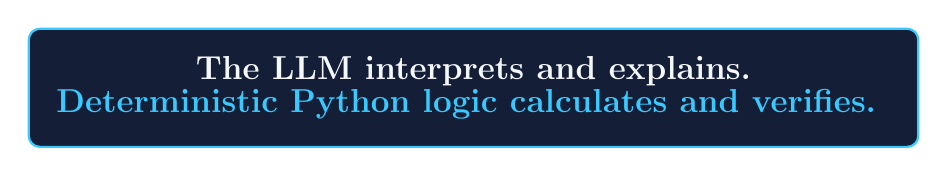
\begin{tikzpicture}
      \node[draw=accentCyan,rounded corners=4pt,fill=panelNavy2,inner sep=10pt,line width=0.8pt,align=center] (principle) {
        \color{textWhite}\large\textbf{The LLM interprets and explains.}\\
        \color{accentCyan}\large\textbf{Deterministic Python logic calculates and verifies.}
      };
    \end{tikzpicture}
  \end{center}
  \vspace{6mm}
  \begin{columns}[t]
    \begin{column}{0.33\textwidth}
      \cardbox{0.92\linewidth}{
        \textcolor{accentBlue}{\textbf{Understand}}\\[1mm]\footnotesize
        Deterministic intent \& entity extraction turns a question (en/hi/hinglish) into a route: search, fare, refund, or policy.
      }
    \end{column}
    \begin{column}{0.33\textwidth}
      \cardbox{0.92\linewidth}{
        \textcolor{accentBlue}{\textbf{Compute \& Retrieve}}\\[1mm]\footnotesize
        Python tools read SQLite directly for every number. RAG retrieves the exact rule/circular section that applies today.
      }
    \end{column}
    \begin{column}{0.33\textwidth}
      \cardbox{0.92\linewidth}{
        \textcolor{accentBlue}{\textbf{Explain \& Confirm}}\\[1mm]\footnotesize
        The response states the real number with its citation. Any change waits for a separate, explicit confirmation.
      }
    \end{column}
  \end{columns}
  \vspace{4mm}
  {\footnotesize\color{textGray}All railway data (stations, trains, fares, bookings) is simulated for this hackathon -- no real IRCTC or railway-system integration.}
\end{frame}

% ======================================================================
\begin{frame}{}
  \framebar{Key Features}{03 -- CAPABILITIES}
  \begin{columns}[t]
    \begin{column}{0.5\textwidth}
      \footnotesize
      \begin{itemize}
        \item Train search \& station-alias resolution \pillDone
        \item Deterministic seat availability \& fare lookup \pillDone
        \item Refund calculation, exact at cut-off boundaries \pillDone
        \item Policy answers grounded in real documents, with citations \pillDone
        \item Circular supersession \& effective-date awareness \pillDone
      \end{itemize}
    \end{column}
    \begin{column}{0.5\textwidth}
      \footnotesize
      \begin{itemize}
        \item English / Hindi / Hinglish query understanding \pillDone
        \item Safe action workflow: preview $\to$ confirm $\to$ execute $\to$ verify \pillPartial
        \item Passenger ownership \& privacy checks \pillDone
        \item Human hand-over for disputes \& safety issues \pillPartial
      \end{itemize}
    \end{column}
  \end{columns}
  \vspace{5mm}
  \cardbox{0.95\linewidth}{\footnotesize\color{textGray}
    \textbf{\color{textWhite}Reading the labels:} \pillDone\ working and tested today. \pillPartial\ designed and wired, with one piece (noted later) still a test fake. Nothing on this slide is end-to-end production-ready -- see Slide 10.
  }
\end{frame}

% ======================================================================
\begin{frame}{}
  \framebar{System Architecture}{04 -- DESIGN}
  \begin{center}
  \resizebox{0.97\textwidth}{!}{%
  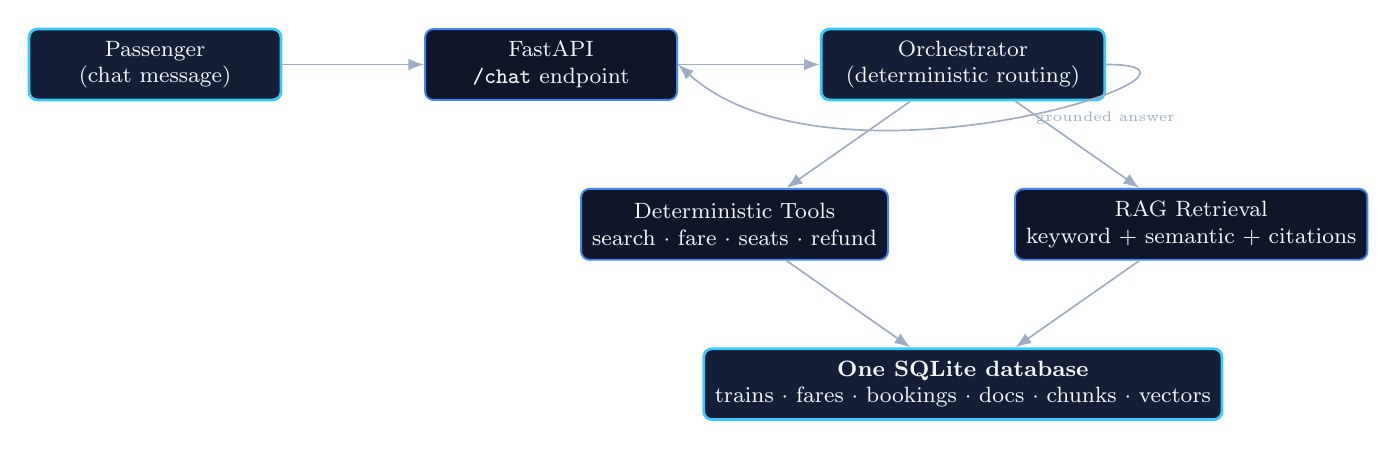
\begin{tikzpicture}[
      node distance=7mm,
      box/.style={draw=accentBlue,rounded corners=3pt,fill=panelNavy,text=textWhite,
                   minimum height=9mm,align=center,font=\footnotesize,line width=0.7pt,inner sep=4pt},
      hl/.style={draw=accentCyan,rounded corners=3pt,fill=panelNavy2,text=textWhite,
                   minimum height=9mm,align=center,font=\footnotesize,line width=1pt,inner sep=4pt},
      arr/.style={-{Latex[length=2mm]},draw=textGray,line width=0.6pt}
    ]
    \node[hl,minimum width=32mm] (passenger) {Passenger\\(chat message)};
    \node[box,minimum width=32mm,right=18mm of passenger] (api) {FastAPI\\\texttt{/chat} endpoint};
    \node[hl,minimum width=36mm,right=18mm of api] (orch) {Orchestrator\\(deterministic routing)};

    \node[box,minimum width=34mm,below=11mm of orch,xshift=-29mm] (tools) {Deterministic Tools\\search $\cdot$ fare $\cdot$ seats $\cdot$ refund};
    \node[box,minimum width=34mm,below=11mm of orch,xshift=29mm] (rag) {RAG Retrieval\\keyword + semantic + citations};

    \node[hl,minimum width=40mm,below=11mm of tools, xshift=29mm] (db) {\textbf{One SQLite database}\\trains $\cdot$ fares $\cdot$ bookings $\cdot$ docs $\cdot$ chunks $\cdot$ vectors};

    \draw[arr] (passenger) -- (api);
    \draw[arr] (api) -- (orch);
    \draw[arr] (orch) -- (tools);
    \draw[arr] (orch) -- (rag);
    \draw[arr] (tools) -- (db);
    \draw[arr] (rag) -- (db);
    \draw[arr] (orch.east) .. controls +(20mm,0) and +(20mm,-18mm) .. (api.east)
       node[midway,right,font=\tiny,text=textGray,xshift=2mm]{grounded answer};
  \end{tikzpicture}%
  }
  \end{center}
  \vspace{3mm}
  \cardbox{0.95\linewidth}{\footnotesize
    \textbf{\color{accentCyan}One} FastAPI app. \textbf{\color{accentCyan}One} SQLite database. \textbf{\color{accentCyan}One} orchestrator. Kept deliberately simple -- every extra moving part has to earn its place.
  }
\end{frame}

% ======================================================================
\begin{frame}{}
  \framebar{Technology Stack}{05 -- STACK}
  \begin{columns}[t]
    \begin{column}{0.5\textwidth}
      \cardbox{0.95\linewidth}{
        \textcolor{accentCyan}{\textbf{Serving \& storage}}\\[1mm]\footnotesize
        \begin{tabular}{@{}ll@{}}
          FastAPI & API layer, \texttt{/chat} endpoint\\
          SQLite & trains, fares, bookings\\
          & documents, chunks, vectors\\
          SQLite FTS5 & keyword (BM25) retrieval\\
        \end{tabular}
      }
      \vspace{4mm}
      \cardbox{0.95\linewidth}{
        \textcolor{accentCyan}{\textbf{Local AI models (Ollama)}}\\[1mm]\footnotesize
        \begin{tabular}{@{}ll@{}}
          \texttt{nomic-embed-text} & embeddings, 768-dim\\
          \texttt{phi3:mini} & local LLM, future use\\
        \end{tabular}
      }
    \end{column}
    \begin{column}{0.5\textwidth}
      \cardbox{0.95\linewidth}{
        \textcolor{accentCyan}{\textbf{Application logic}}\\[1mm]\footnotesize
        \begin{itemize}
          \item Python -- all deterministic calculations
          \item Regex/keyword-based intent \& entity extraction
          \item Reciprocal Rank Fusion for hybrid retrieval
        \end{itemize}
      }
      \vspace{4mm}
      \cardbox{0.95\linewidth}{
        \textcolor{accentCyan}{\textbf{Quality}}\\[1mm]\footnotesize
        \begin{itemize}
          \item pytest -- 145+ automated tests, run continuously
          \item A reusable Recall@k / MRR evaluation harness
        \end{itemize}
      }
    \end{column}
  \end{columns}
\end{frame}

% ======================================================================
\begin{frame}{}
  \framebar{RAG Pipeline -- Deep Dive}{06 -- RAG}
  \begin{center}
  
\begin{tikzpicture}[
      node distance=5mm,
      pstep/.style={draw=accentBlue,rounded corners=3pt,fill=panelNavy,text=textWhite,
                    minimum height=13mm,minimum width=22mm,align=center,font=\tiny,line width=0.7pt,inner sep=3pt},
      arr/.style={-{Latex[length=2mm]},draw=accentCyan,line width=0.8pt}
    ]
    \node[pstep] (p1) {Markdown\\documents};
    \node[pstep,right=of p1] (p2) {Metadata\\extraction};
    \node[pstep,right=of p2] (p3) {Section-aware\\chunking};
    \node[pstep,right=of p3] (p4) {Embedding\\(nomic-embed-text)};
    \node[pstep,right=of p4] (p5) {SQLite\\storage};
    \foreach \a/\b in {p1/p2,p2/p3,p3/p4,p4/p5} \draw[arr] (\a) -- (\b);
  \end{tikzpicture}
  \end{center}
  \vspace{5mm}
  \begin{columns}[t]
    \begin{column}{0.48\textwidth}
      \cardbox{0.95\linewidth}{
        \textcolor{accentCyan}{\textbf{Corpus generated}}\\[1mm]\footnotesize
        \begin{tabular}{@{}lr@{}}
          Documents & 38 \\
          \quad rules / circulars / FAQs & 12 / 6 / 20 \\
          Chunks (section-aware) & 105 \\
          Real embeddings generated & 104 \\
          Embedding dimension & 768 \\
        \end{tabular}
      }
    \end{column}
    \begin{column}{0.48\textwidth}
      \cardbox{0.95\linewidth}{
        \textcolor{warnAmber}{\textbf{A real implementation lesson}}\\[1mm]\footnotesize
        One chunk's text came out empty because of a malformed heading split across two lines in the source document. It was \textbf{skipped and reported}, never faked with a placeholder vector.
      }
    \end{column}
  \end{columns}
\end{frame}

% ======================================================================
\begin{frame}{}
  \framebar{Hybrid Search and Embeddings}{07 -- RETRIEVAL}
  \begin{columns}[t]
    \begin{column}{0.46\textwidth}
      \cardbox{0.95\linewidth}{
        \textcolor{accentCyan}{\textbf{Two retrieval legs, fused}}\\[1mm]\footnotesize
        \begin{itemize}
          \item \textbf{Keyword}: SQLite FTS5, BM25 scoring
          \item \textbf{Semantic}: cosine similarity over 768-dim embeddings
          \item \textbf{Fusion}: Reciprocal Rank Fusion combines both rankings
        \end{itemize}
      }
      \vspace{4mm}
      \cardbox{0.95\linewidth}{
        \textcolor{accentCyan}{\textbf{Tested across languages}}\\[1mm]\footnotesize
        English, Hindi and Hinglish queries -- including paraphrases with \emph{no literal keyword overlap} at all (e.g. asking about ``a small dog in a private compartment'' still finds the pet policy).
      }
    \end{column}
    \begin{column}{0.5\textwidth}
      \cardbox{0.97\linewidth}{
        \textcolor{accentCyan}{\textbf{Effective-date \& supersession, verified live}}\\[1.5mm]\footnotesize
        \begin{tabular}{@{}p{0.42\linewidth}p{0.42\linewidth}@{}}
          \textbf{Before 10 Dec 2026} & \textbf{From 10 Dec 2026}\\
          Earlier circular's refund rate wins & Newer circular takes precedence\\
        \end{tabular}
        \vspace{1.5mm}\\
        Superseded or not-yet-effective sources are \textbf{excluded and flagged} in the response -- never silently dropped, never silently applied early.
      }
      \vspace{4mm}
      \cardbox{0.95\linewidth}{
        \footnotesize Every retrieved answer carries a \textcolor{accentCyan}{\textbf{citation}}: document ID + exact section.
      }
    \end{column}
  \end{columns}
\end{frame}

% ======================================================================
\begin{frame}{}
  \framebar{Deterministic Backend Tools}{08 -- TOOLS}
  \begin{columns}[t]
    \begin{column}{0.4\textwidth}
      \cardbox{0.95\linewidth}{
        \textcolor{accentCyan}{\textbf{Five tools, all pure Python}}\\[1mm]\footnotesize
        \begin{itemize}
          \item Station resolution (names \& aliases)
          \item Train search
          \item Seat availability
          \item Fare calculation
          \item Refund calculation
        \end{itemize}
        \vspace{1mm}
        None of these are ever delegated to the LLM.
      }
    \end{column}
    \begin{column}{0.58\textwidth}
      \cardbox{0.97\linewidth}{
        \textcolor{accentCyan}{\textbf{Worked example (simulated data)}}\\[1.5mm]\footnotesize
        Pune $\to$ Nagpur, Train \textbf{12123 ``Ujjwal Express''}\\
        Departs 18:40 $\cdot$ Arrives 06:10 (next day)\\
        2AC availability: \textbf{9 / 10} seats free $\cdot$ Fare: \textbf{Rs 2{,}040}
      }
      \vspace{3mm}
      \cardbox{0.97\linewidth}{
        \textcolor{accentCyan}{\textbf{Refund boundary example}}\\[1.5mm]\footnotesize
        Exactly 48h before departure: charge \textbf{Rs 200} $\to$ refund \textbf{Rs 1{,}840}\\
        One minute later: the \emph{next} refund bracket applies (higher charge)
      }
    \end{column}
  \end{columns}
  \vspace{4mm}
  {\footnotesize\color{textGray}Simulated project example -- no real IRCTC or railway-system integration.}
\end{frame}

% ======================================================================
\begin{frame}{}
  \framebar{Safety, Privacy and Reliability}{09 -- SAFETY}
  \begin{columns}[t]
    \begin{column}{0.5\textwidth}
      \footnotesize
      \begin{itemize}
        \item Passenger identity injected server-side via \texttt{X-Passenger-Id} -- never read from chat text \pillDone
        \item A passenger can never see another passenger's booking; non-existent and foreign bookings get the \emph{identical} refusal \pillDone
        \item The LLM never determines a fare, seat or refund amount \pillDone
        \item A booking change never executes just because it was asked for \pillPartial
      \end{itemize}
    \end{column}
    \begin{column}{0.5\textwidth}
      \footnotesize
      \begin{itemize}
        \item Preview and confirmation are two separate, explicit steps \pillPartial
        \item Circulars supersede older rules automatically from their effective date \pillDone
        \item Untrusted retrieved content is treated as data, never as an instruction \pillDone
        \item Sensitive disputes and safety reports are routed to a human \pillPartial
      \end{itemize}
    \end{column}
  \end{columns}
  \vspace{5mm}
  \cardbox{0.96\linewidth}{\footnotesize
    \textbf{\color{warnAmber}Honest status:} the confirmation step and the human hand-over step are both designed and wired into the orchestrator, but today's \texttt{ActionService} and \texttt{HandoffService} are \pillMock\ -- real backend execution is upcoming work (Slide 14), not yet connected end to end.
  }
\end{frame}

% ======================================================================
\begin{frame}{}
  \framebar{End-to-End User Journey}{10 -- DEMO FLOW}
  \begin{center}
  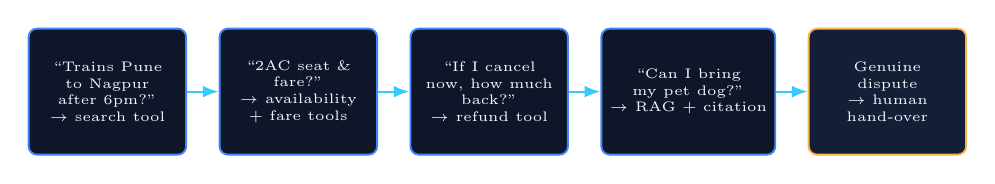
\begin{tikzpicture}[
      node distance=4mm,
      flowstep/.style={draw=accentBlue,rounded corners=3pt,fill=panelNavy,text=textWhite,
                   minimum height=16mm,minimum width=20mm,align=center,font=\tiny,line width=0.7pt,inner sep=3pt},
      arr/.style={-{Latex[length=2mm]},draw=accentCyan,line width=0.8pt}
    ]
    \node[flowstep] (s1) {``Trains Pune\\to Nagpur\\after 6pm?''\\$\to$ search tool};
    \node[flowstep,right=of s1] (s2) {``2AC seat \&\\fare?''\\$\to$ availability\\+ fare tools};
    \node[flowstep,right=of s2] (s3) {``If I cancel\\now, how much\\back?''\\$\to$ refund tool};
    \node[flowstep,right=of s3] (s4) {``Can I bring\\my pet dog?''\\$\to$ RAG + citation};
    \node[flowstep,right=of s4,fill=panelNavy2,draw=warnAmber] (s5) {Genuine\\dispute\\$\to$ human\\hand-over};
    \foreach \a/\b in {s1/s2,s2/s3,s3/s4,s4/s5} \draw[arr] (\a) -- (\b);
  \end{tikzpicture}
  \end{center}
  \vspace{5mm}
  \cardbox{0.96\linewidth}{\footnotesize
    Every step above uses a \textbf{real} tool call or a \textbf{real} retrieved citation -- the numbers and documents shown in this flow are not hand-written placeholders, they come from the actual SQLite data and the actual RAG pipeline.
  }
\end{frame}

% ======================================================================
\begin{frame}{}
  \framebar{Evaluation and Results}{11 -- RESULTS}
  \begin{columns}[t]
    \begin{column}{0.44\textwidth}
      \cardbox{0.97\linewidth}{
        \textcolor{accentCyan}{\textbf{RAG retrieval metrics}}\\[1.5mm]\footnotesize
        Scored on 21 questions (from a 34-question evaluation set) that carry a real document-citation ground truth.
        \vspace{2mm}\\
        \begin{tabular}{@{}lr@{}}
          \textbf{Recall@5} & \textbf{0.571} (12/21)\\
          \textbf{MRR} & \textbf{0.293}\\
        \end{tabular}
      }
    \end{column}
    \begin{column}{0.54\textwidth}
      \cardbox{0.97\linewidth}{
        \textcolor{accentCyan}{\textbf{What these numbers mean, honestly}}\\[1mm]\footnotesize
        \textbf{Recall@5}: the correct document was in the top 5 results for about 57\% of ground-truth questions.\\[1mm]
        \textbf{MRR} of 0.293: when the correct citation did appear, it typically was \emph{not} ranked first. This is a modest, working baseline -- not an exceptional result -- and a known target for further tuning.
      }
    \end{column}
  \end{columns}
  \vspace{4mm}
  \cardbox{0.96\linewidth}{\footnotesize
    \textbf{\color{accentCyan}Also verified directly:}\ real Ollama embedding generation (768-dim, 104 vectors) $\cdot$ idempotent document re-ingestion (no duplicates on re-run) $\cdot$ supersession/effective-date behaviour changing the live answer at the right date.
  }
\end{frame}

% ======================================================================
\begin{frame}{}
  \framebar{Challenges and Technical Learnings}{12 -- LEARNINGS}
  \footnotesize
  \begin{itemize}
    \item A malformed document heading silently produced one empty chunk -- taught us to validate chunk boundaries, not just assume well-formed input.
    \item Correctly overriding an older rule with a newer circular, \emph{only from its effective date}, needed careful cluster-based resolution logic -- not a simple ``newest wins'' rule.
    \item Keyword (BM25) and semantic (cosine) scores live on completely different scales -- fusing them meaningfully needed Reciprocal Rank Fusion rather than a naive weighted average.
    \item The hardest discipline was architectural, not algorithmic: \emph{never} letting the LLM touch money or seat arithmetic, even where it would have been easier to let it ``just answer.''
    \item All data -- stations, trains, fares, bookings, passengers -- is simulated; none of it reflects a real railway system.
  \end{itemize}
\end{frame}

% ======================================================================
\begin{frame}{}
  \framebar{Future Scope and Conclusion}{13 -- NEXT}
  \begin{columns}[t]
    \begin{column}{0.52\textwidth}
      \cardbox{0.95\linewidth}{
        \textcolor{accentCyan}{\textbf{Future scope}}\\[1mm]\footnotesize
        \begin{itemize}
          \item Real LLM-based response composition (currently deterministic/templated, not generative) \pillFuture
          \item Replace the \texttt{FakeActionService} / \texttt{FakeHandoffService} test fakes with real backend execution \pillFuture
          \item Connect \texttt{/ingest} fully to live RAG re-indexing \pillFuture
          \item A dedicated booking-status tool \pillFuture
          \item Broaden the evaluation set and re-tune retrieval fusion \pillFuture
        \end{itemize}
      }
    \end{column}
    \begin{column}{0.44\textwidth}
      \cardbox{0.95\linewidth}{
        \textcolor{accentCyan}{\textbf{Conclusion}}\\[1mm]\footnotesize
        We built and tested a working foundation: deterministic money/seat calculations that never guess, a grounded RAG pipeline with real citations and supersession awareness, and a safety-first action design -- with an honest, specific roadmap for what's left to connect end to end.
      }
    \end{column}
  \end{columns}
  \vspace{3mm}
  \begin{center}
    {\large\color{accentCyan}\textbf{Thank you.}}\quad{\footnotesize\color{textGray}Questions welcome.}
  \end{center}
\end{frame}

\end{document}
